\section{Cambios y Olvidos de Contraseñas}

Mantener tu clave unificada y protegida es prioritario en materia de sistemas al operar de manera interactiva expedientes de salud que te delegan. Si dejaste de utilizar la plataforma y olvidaste las claves o te han comunicado alertas de usurpación de correo, tienes capacidad resolutiva.

\subsection{Recuperación al Olvidar Contraseña (Sin Iniciar Sesión)}
Si no puedes entrar en absoluto a tu cuenta porque perdiste tus datos de acceso:
\begin{enumerate}
    \item Ve hasta la página general de inicio de sesión de RadiographXpress.
    \item Debajo y alejado del botón principal azul para loggearte, haz clic en el hipervínculo rosa que formula la pregunta \textbf{"¿Olvidaste tu contraseña?"}.
    \item Se habilitará una nueva vista y un campo vacío en un recuadro, donde debes escribir el \textbf{correo electrónico asociado a tu cuenta de sistema de Médico Asociado}.
    \item Presiona el botón verde oscuro/teal de "Enviar mi enlace recuperación".
    \item Luego de unos segundos, se te enviará un correo a la dirección de tu cuenta.
    \begin{figure}[H]
        \centering
        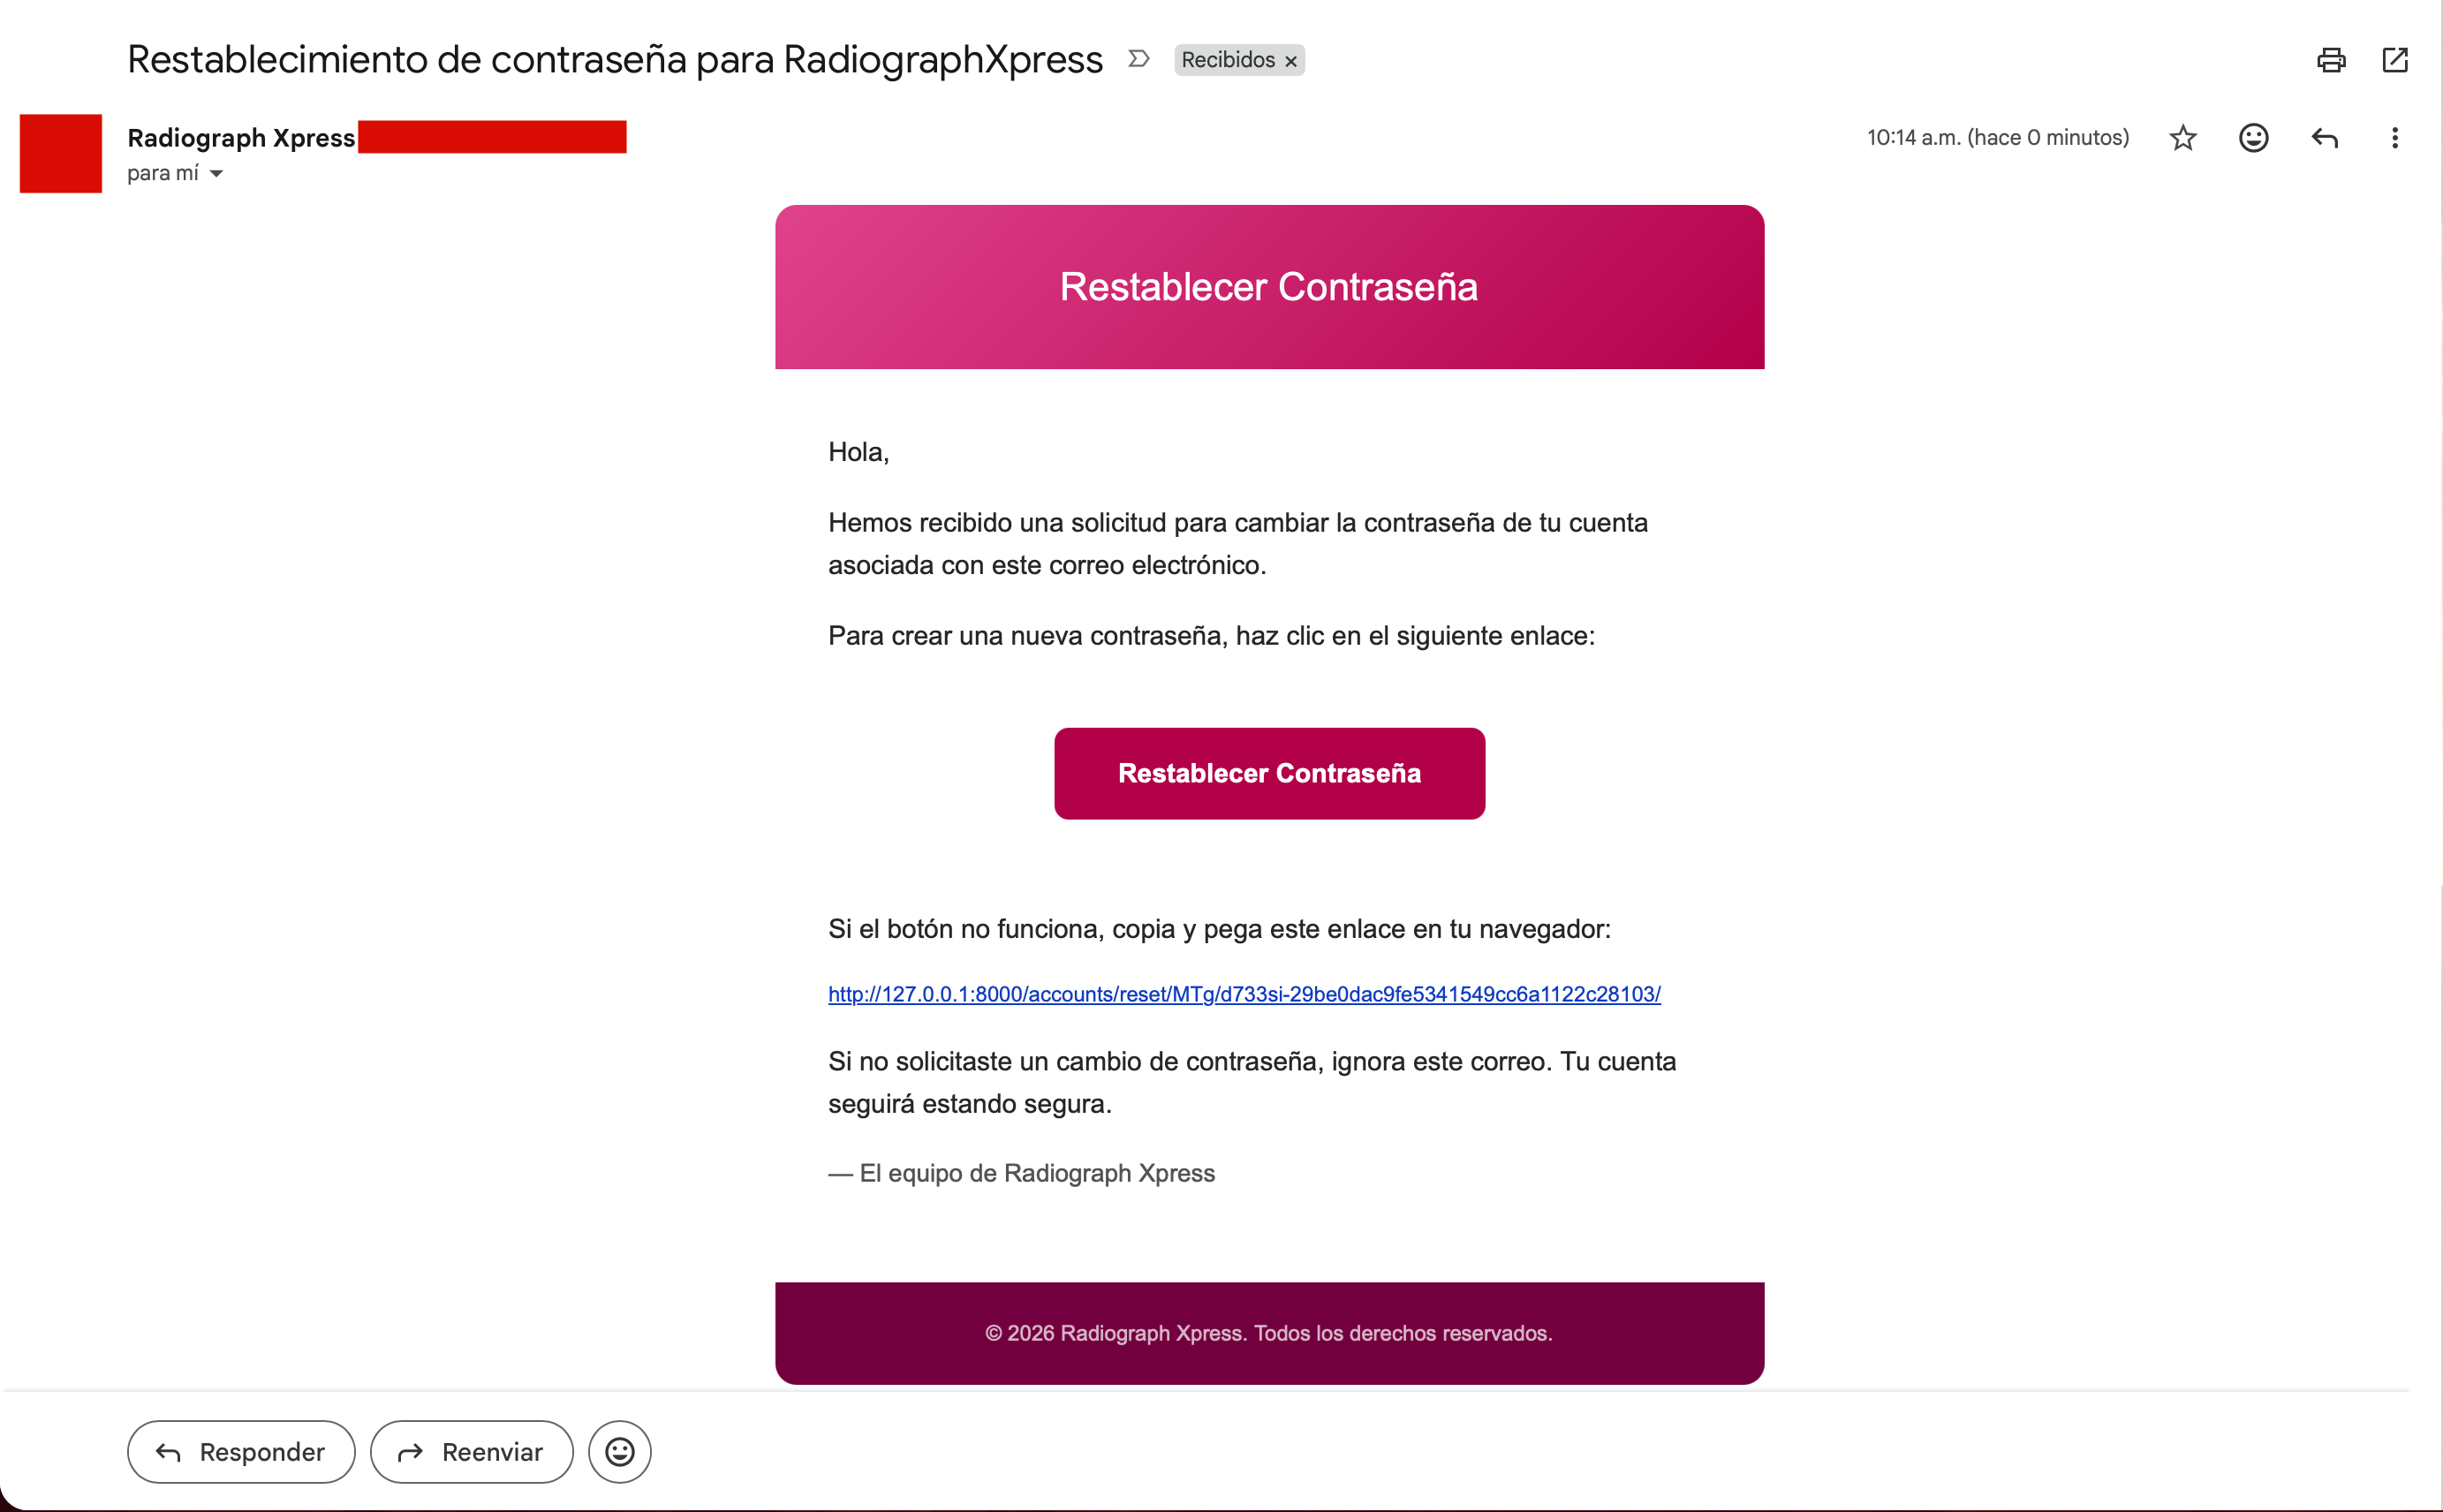
\includegraphics[width=0.7\textwidth]{screenshots/password_reset.png}
        \caption{Email con el enlace automático para la restitución de cuenta.}
    \end{figure}
    \item En tu buzón de entrada localizarás un mensaje automático cuyo título es "Restablecimiento de contraseña". \textit{Considera investigar en áreas no deseadas/spam}. 
    \item En el centro del correo, presiona en el botón de color contrastante de que dice \textbf{"Restablecer Contraseña"} el cual redirige a una liga de seguridad cifrada especial. (Solo tiene vigencia activa y segura por corto plazo).
    \item El link abrirá y lanzará una pestaña de nuestro sistema, brindando una zona de escritura para "Nueva Clave". Ingresa los dígitos y signos que vas a implementar de aquí adelante (deben superar tu vieja robustez) e ingresalas nuevamente para corroborar igualidad.
    \item  Haz clic en \textbf{"Guardar y Terminar"} o "Cambiar mi contraseña". Regresarás al Inicio predeterminado; \textit{Intenta loggearte con tus credenciales reconstruidas para confirmar éxito}.
\end{enumerate}
